%laden der Präambel mit Latexbefehlen/-klassen
% !TeX encoding = UTF-8
% !TeX spellcheck = es_MX

%Clase de documento, configuración de idioma, fuentes
\documentclass[a1paper,portrait,fontscale=0.40]{baposter}
\usepackage[spanish,es-tabla]{babel}
\usepackage[utf8]{inputenc}
\usepackage{arev}
\usepackage[T1]{fontenc}

%Matemáticas, símbolos
\usepackage{amsmath}
\usepackage{amssymb}

%Tipografía
\usepackage[auto]{microtype}

%Inclusión de imágenes, tablas, código fuente
\usepackage{graphicx}
\usepackage{booktabs}
\usepackage{multirow}
\usepackage{array}
\usepackage{paralist}
\usepackage{pifont}

%Colores y TikZ
\usepackage{xcolor}
\usepackage{colortbl}
\usepackage{tikz}
\usetikzlibrary{arrows.meta,positioning,shapes.geometric,backgrounds,fit,calc}

%Búsqueda de gráficos (las figuras/logos se reutilizan desde docs/poster/)
\graphicspath{{../sem_tesis4/figures/}{../../reports/Tesis/logo/}{../../reports/Tesis/figures/}{../../reports/}{bilder/}}

%Paleta del proyecto (de sem_tesis4 / poster navy-cream, con acento lila)
\definecolor{cream}{HTML}{F2EEE3}
\definecolor{paper}{HTML}{FBFAF6}
\definecolor{navy}{HTML}{2F3E4E}
\definecolor{accentA}{HTML}{7E57C2}
\definecolor{accentB}{HTML}{EF6C00}
\definecolor{accentC}{HTML}{2E7D32}
\definecolor{accentD}{HTML}{C62828}
\definecolor{rule}{HTML}{B5AFA1}

%Definición de colores (degradado lila en encabezados: blanco -> lila, marco negro)
\definecolor{standardfontcolor}{HTML}{2F3E4E}
\definecolor{bordercol}{HTML}{000000}
\definecolor{headercol1}{HTML}{FFFFFF}
\definecolor{headercol2}{HTML}{7E57C2}
\definecolor{headerfontcol}{HTML}{000000}
\definecolor{boxcolor}{HTML}{FBFAF6}

%Macro auxiliar para resaltar
\newcommand{\hl}[1]{{\color{accentD}\textbf{#1}}}

%Colores para los perfiles de aspectos (azul = Pueblo A, rosa = Pueblo B)
\definecolor{azulperfil}{HTML}{3B3FA8}
\definecolor{rosaperfil}{HTML}{C42B86}

%Diagrama de radar/red para los perfiles de aspectos de los pueblos.
% [#1] Opacidad del relleno (opcional, default 0.85)
%  #2  Título,  #3 Color,
%  #4..#8 Valores (Gastronomía, Naturaleza, Cultura, Tranquilidad, Precio) en escala 0-5.
\newcommand{\perfilradar}[8][0.85]{%
	\begin{tikzpicture}[every node/.style={font=\footnotesize}]
		\def\maxR{2.6}
		% Pentágonos concéntricos (rejilla)
		\foreach \r in {1,...,5}{
				\draw[navy!90,line width=0.4pt]
				(90:{\r/5*\maxR}) -- (18:{\r/5*\maxR}) -- (-54:{\r/5*\maxR}) --
				(-126:{\r/5*\maxR}) -- (162:{\r/5*\maxR}) -- cycle;
			}
		% Ejes
		\foreach \a in {90,18,-54,-126,162}{
				\draw[navy!35,line width=0.4pt] (0,0) -- (\a:\maxR);
			}
		% Polígono de datos con degradado radial (claro al centro -> intenso en el borde)
		\begin{scope}
			\clip (90:{#4/5*\maxR}) -- (18:{#5/5*\maxR}) -- (-54:{#6/5*\maxR}) --
			(-126:{#7/5*\maxR}) -- (162:{#8/5*\maxR}) -- cycle;
			\shade[inner color=#3!12,outer color=#3!85,opacity=#1] (0,0) circle (\maxR);
		\end{scope}
		\draw[draw=#3,line width=1.3pt,opacity=#1]
		(90:{#4/5*\maxR}) -- (18:{#5/5*\maxR}) -- (-54:{#6/5*\maxR}) --
		(-126:{#7/5*\maxR}) -- (162:{#8/5*\maxR}) -- cycle;
		% Círculo central con el promedio
		\fill[paper] (0,0) circle (0.74cm);
		\draw[navy!35,line width=0.4pt] (0,0) circle (0.74cm);
		\node[align=center] at (0,0) {Promedio:\\4.5};
		% Etiquetas de los ejes (radio mayor para separar del vértice)
		\pgfmathsetmacro{\labelR}{\maxR+0.14}
		\node[above]       at (90:\labelR)   {Gastronom\'ia};
		\node[right]       at (18:\labelR)   {Ambiente};
		\node[below right] at (-54:\labelR)  {Servicio};
		\node[below left]  at (-126:\labelR) {Infrastructura};
		\node[left]        at (162:\labelR)  {Precio};
		% Título
		\node[font=\normalsize\bfseries,text=#3] at (90:{\maxR+1.05}) {#2};
	\end{tikzpicture}%
}


\begin{document}
\typeout{Poster rendering started}

\color{standardfontcolor}

\begin{poster}{
		grid=false,
		columns=2,
		%colspacing=length
		headerheight=0.12\textheight,
		eyecatcher=false,
		borderColor=bordercol,
		headerColorOne=headercol1,
		headerColorTwo=headercol2,
		headerFontColor=headerfontcol,
		boxColorOne=boxcolor,
		headershape=roundedright,
		headerfont=\sffamily\bfseries\large,
		headershade=shadelr,
		textborder=rectangle,
		headerborder=closed,
		boxshade=plain,
		background=none
	}
	%%% Eye Catcher %%%%%%%%%%%%%%%%%%%%%%%%%%%%%%%%%%%%%%%%%%%%%%%%%%%%%%%%%%%%%%%
	{
		Eye Catcher, empty if option eyecatcher=false - unused
	}
	%----------------------------------------------------------------------------------------
	%	TITLE AND AUTHOR NAME
	%----------------------------------------------------------------------------------------
	%
	{
		\textsf %Sans Serif
		{\Large Sistema de Recomendaci\'on H\'ibrido para Pueblos M\'agicos:\\ Integrando Análisis de Sentimientos Basado en Aspectos}
	}
	{\sf\vspace{0.4em}\\
		\small Gustavo Hern\'andez Angeles\quad$\cdot$\quad
		\textbf{Asesor:} Dr.\ Norberto A.\ Hern\'andez Leandro\quad$\cdot$\quad\newline
		\textbf{Comit\'e:} Dr.\ Alejandro Rosales P\'erez, Dr.\ Miguel \'A.\ \'Alvarez Carmona
		\vspace{0.3em}\\
		\footnotesize \textbf{CIMAT Monterrey} — Centro de Investigaci\'on en Matem\'aticas, Unidad Monterrey\,$\cdot$\,Alianza Centro 502, 66629, Apodaca, Nuevo Le\'on
	}
	% University/lab logo
	{
\includegraphics[height=2.7cm]{LOGOTIPO_SIN_FONDO-02.png}}
	%
	%----------------------------------------------------------------------------------------
	%	1. EL PROBLEMA
	%----------------------------------------------------------------------------------------
	\headerbox{1.\ Introducción}{name=problema,column=0,row=0,span=2}{
		El programa \textbf{Pueblos M\'agicos} re\'une destinos tur\'isticos con
		atractivos culturales, gastron\'omicos y naturales muy diversos.
		Ante esta \hl{amplia gama de opciones}, el viajero enfrenta el problema
		cl\'asico de sobrecarga de informaci\'on.
		\vskip0.2ex
		\begin{center}\itshape
			\textbf{Objetivo:} dise\~nar un sistema de recomendaci\'on h\'ibrido que, utilizando el Análisis Basado en Aspectos (ABSA),
			combine el filtrado colaborativo y el filtrado basado en contenido,
			\textbf{personalizando} la selecci\'on del siguiente Pueblo M\'agico
			seg\'un las preferencias latentes de cada usuario.
		\end{center}
	}

	%----------------------------------------------------------------------------------------
	%	2. DATOS
	%----------------------------------------------------------------------------------------
	\headerbox{2.\ Datos: REST-MEX 2025}{name=datos,column=0,below=problema,span=1}{
		\begin{compactitem}\setlength\itemsep{2pt}
			\item {\bfseries\normalsize\color{accentA}79{,}264} rese\~nas
			\item {\bfseries\normalsize\color{accentB}9{,}582} usuarios
			\item {\bfseries\normalsize\color{accentC}48} Pueblos M\'agicos
		\end{compactitem}
		\vskip0.3ex
		\centering\scriptsize
		\renewcommand{\arraystretch}{1.2}
		\setlength{\tabcolsep}{3pt}
		\begin{tabular}{@{}l c c l l l p{2.0cm}@{}}
			\toprule
			\textbf{Calif.} & \textbf{Fecha} & \textbf{Pueblo} & \textbf{Tipo} & \textbf{Lugar}  & \textbf{Review}                               \\
			\midrule
			5.0             & 2023-08        & Tulum           & Attractive    & Ruinas de Tulum & \textit{``El ambiente es incre\'ible\ldots''} \\
			\bottomrule
		\end{tabular}
		\vspace{0.3cm}

		\footnotesize La separación entre conjuntos de entrenamiento y prueba se realizó utilizando partici\'on temporal \emph{last-month-out} por usuario, resultando en una proporción 70-30, en promedio.
	}

	%----------------------------------------------------------------------------------------
	%	6. CREACION DE PERFILES
	%----------------------------------------------------------------------------------------
	\headerbox{6.\ Creaci\'on de perfiles}{name=perfiles,column=1,below=problema,span=1}{
		Cada fila de las matrices estructurales es un \textbf{perfil interpretable}
		por aspecto: $X_u$ (importancia del usuario) y $Y_p$ (calidad del pueblo).
		\vskip0.3ex
		\centering
		\resizebox{0.8\linewidth}{!}{%
			\perfilradar{Pueblo M\'agico 3}{azulperfil}{3.5}{5}{5}{4.0}{3.0}%
			\hspace{0.6cm}%
			\perfilradar{Usuario 1}{rosaperfil}{4.5}{3}{5}{3}{2.5}%
		}
		\vskip0.3ex
		\raggedright\footnotesize
		ABSA construye perfiles por aspecto tanto para \emph{pueblos} ($Y_p$, calidad)
		como para \emph{usuarios} ($X_u$, importancia). El pueblo destaca en
		servicio y ambiente; el usuario \hl{prioriza} gastronom\'ia y servicio. Recomendar
		consiste en \textbf{emparejar} ambos perfiles, recuperando la informaci\'on que
		la calificaci\'on media oculta.
	}

	%----------------------------------------------------------------------------------------
	%	7. MODELO HIBRIDO
	%----------------------------------------------------------------------------------------
	\headerbox{7.\ Modelo h\'ibrido}{name=modelo,column=1,below=perfiles,span=1}{
		Dos modelos se ajustan \emph{una vez}; cada $\alpha$ s\'olo re-pondera:
		\vskip0.2ex
		\begin{center}
			\setlength{\fboxsep}{4pt}
			\colorbox{accentD!15}{$\displaystyle
					\hat y_{u,p}(\alpha)=\alpha\,\hat y^{\mathtt{CF}}_{u,p}
					+(1-\alpha)\,\hat y^{\mathtt{CB}}_{u,p}$}
		\end{center}
		\vskip0.2ex
		Objetivo que pondera relevancia y diversidad:
		\[
			f(\alpha)=\beta\,\mathrm{NDCG@K}(\alpha)+(1-\beta)\,\mathrm{Cov@K}(\alpha),\quad
			\alpha\in[0,1].
		\]
	}

	%----------------------------------------------------------------------------------------
	%	4. ARQUITECTURA DEL SISTEMA
	%----------------------------------------------------------------------------------------
	\headerbox{3.\ Arquitectura del sistema}{name=arquitectura,column=0,below=datos,span=1}{
		\centering
		\scalebox{0.42}{%
			\begin{tikzpicture}[
				node distance=10mm,
				every node/.style={font=\large},
				data/.style={rounded corners=6pt,draw=navy,line width=1.1pt,fill=cream,
						align=center,minimum width=7.0cm,minimum height=2.0cm},
				proc/.style={rounded corners=6pt,draw=accentA,line width=1.6pt,fill=accentA!12,
						align=center,minimum width=7.0cm,minimum height=2.2cm},
				mat/.style={rounded corners=6pt,draw=accentC,line width=1.4pt,fill=accentC!12,
						align=center,minimum width=3.2cm,minimum height=1.9cm},
				mod/.style={rounded corners=6pt,draw=accentB,line width=1.6pt,fill=accentB!14,
						align=center,minimum width=7.2cm,minimum height=2.2cm},
				fus/.style={rounded corners=6pt,draw=accentD,line width=1.8pt,fill=accentD!12,
						align=center,minimum width=9.0cm,minimum height=2.2cm},
				flow/.style={-{Stealth[length=5mm]},line width=1.4pt,navy}]

				\node[data] (ds) {\textbf{REST-MEX Dataset}\\\normalsize reseñas + calificaciones};
				\node[proc,below=of ds] (absa) {\textbf{ABSA}\\\normalsize aspecto + sentimiento};

				\node[mat,below left=14mm and -3.4cm of absa] (mx) {$X$\\\normalsize usuario--aspecto};
				\node[mat,right=4mm of mx] (my) {$Y$\\\normalsize pueblo--aspecto};
				\node[mat,left=4mm of mx] (ma) {$A$\\\normalsize rating};

				\node[mod,below left=17mm and 1.5cm of mx] (att)
				{\textbf{Modelo Colaborativo}\\\normalsize sim.\ usuario-usuario en $X$};
				\node[mod,below right=17mm and 1.5cm of mx] (qual)
				{\textbf{Modelo Basado en Contenido}\\\normalsize emparejamiento $X{\cdot}Y$};

				\node[fus] (fus) at ($(att.south)!0.5!(qual.south)+(0,-15mm)$)
				{\textbf{Fusi\'on convexa}\\\normalsize $\hat y=\alpha\,\hat y^{\mathrm{CF}}+(1{-}\alpha)\,\hat y^{\mathrm{CB}}$};

				\draw[flow] (ds) -- (absa);
				\draw[flow] (absa.south) -- ($(mx.north)+(0,0.0)$);
				\draw[flow] (absa.south) -- (my.north);
				\draw[flow] (ds.west) to[out=180,in=90] (ma.north);
				\draw[flow] (ma.south) to[out=270,in=60] (att.north);
				\draw[flow] (mx.south) to[out=245,in=15] (att.north);
				\draw[flow] (mx.south) to[out=295,in=165] (qual.north);
				\draw[flow] (my.south) to[out=270,in=120] (qual.north);
				\draw[flow] (att.south) to[out=270,in=180] (fus.west);
				\draw[flow] (qual.south) to[out=270,in=0] (fus.east);
			\end{tikzpicture}}
		\vskip0.2ex
		\raggedright\footnotesize
		Las se\~nales ABSA alimentan las matrices estructurales; dos modelos basados en
		aspectos se combinan en un h\'ibrido de un solo par\'ametro.
	}

	%----------------------------------------------------------------------------------------
	%	3. PIPELINE ABSA
	%----------------------------------------------------------------------------------------
	\headerbox{4. ABSA}{name=pipeline,column=0,below=arquitectura,span=1}{
		Cada rese\~na se segmenta en oraciones y se procesa con dos modelos \emph{transformer}:
		\begin{compactitem}\setlength\itemsep{0pt}
			\vspace{0.2cm}
			\item \textbf{Aspecto}: se utiliza la clasificación zero-shot mediante NLI para la clasificación de aspecto.
			\item \textbf{Sentimiento}: se utiliza un modelo tipo BERT para la clasificación de sentimiento, en una escala de 1-5.
			\vspace{0.2cm}
		\end{compactitem}
		Los aspectos considerados en este proyecto fueron: servicio, precio, ambiente, gastronomía, ubicación e infraestructura.

	}

	%----------------------------------------------------------------------------------------
	%	5. MATRICES ESTRUCTURALES
	%----------------------------------------------------------------------------------------
	\headerbox{5.\ Matrices estructurales}{name=matrices,column=0,below=pipeline,span=1}{
	A partir de ABSA se construyen tres matrices:
	% \vskip0.2ex
	\begin{gather*}
		X_{u,j}=1+(N-1)\!\left(\tfrac{2}{1+e^{-t_{uj}/T_x}}-1\right),
		\quad
		Y_{p,j}=1+\tfrac{N-1}{1+e^{-\bar{s}_{pj}/T_y}}\\[3pt]
		A_{u,p}=\tfrac{1}{|\mathcal{R}_{u,p}|}\!\sum_{r\in\mathcal{R}_{u,p}}\!\text{rating}(r)
	\end{gather*}
	{\footnotesize\centering
	\renewcommand{\arraystretch}{1.0}
	\begin{tabular}{@{}c l l@{}}
		\toprule
		\textbf{Matriz} & \textbf{Forma}             & \textbf{Significado}        \\
		\midrule
		$A$             & usuarios $\times$ pueblos  & calificaci\'on media        \\
		$X$             & usuarios $\times$ aspectos & importancia usuario-aspecto \\
		$Y$             & pueblos $\times$ aspectos  & calidad pueblo-aspecto      \\
		\bottomrule
	\end{tabular}\par}
	\vskip0.2ex

	}

	%----------------------------------------------------------------------------------------
	%	7. ABLACION DE X Y Y
	%----------------------------------------------------------------------------------------
	% \headerbox{7.\ Ablaci\'on de $X$ y $Y$}{name=ablacion,column=1,below=modelo,span=1}{
	% 	Dise\~no factorial de las modificaciones sobre Zhang et al.\ (2014)
	% 	(variantes A--D). \texttt{CBQuality} a $K{=}10$:
	% 	\vskip0.2ex
	% 	\centering
	% 	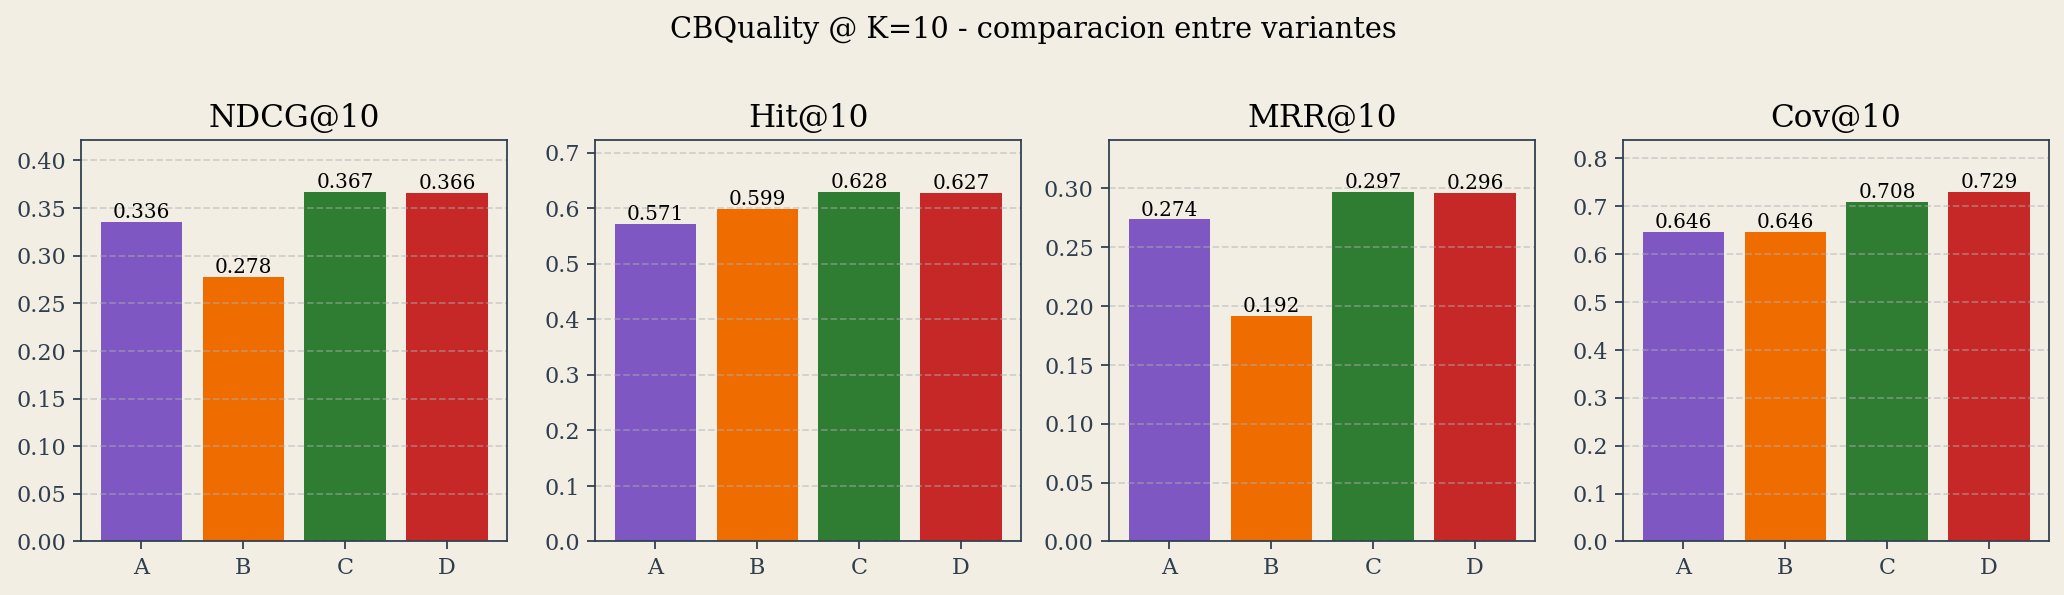
\includegraphics[width=0.52\textwidth]{summary_k10.png}
	% 	\vskip0.3ex
	% 	\raggedright
	% 	\begin{compactitem}\setlength\itemsep{0pt}
	% 		\item En \textbf{B}, $Y$ \hl{satura} ($97.9\%$ de celdas $>4.5$): NDCG cae a $0.278$.
	% 		\item El escalamiento $T$ (C, D) \textbf{recupera la discriminaci\'on}:
	% 		$+9$ pts de NDCG y $+6$ de cobertura.
	% 		\item \textbf{Decisi\'on:} se adopta la variante \textbf{D} ($T$ en ambas
	% 		matrices; se descarta el $\log$).
	% 	\end{compactitem}
	% }

	%----------------------------------------------------------------------------------------
	%	8. TRADE-OFF relevancia VS COBERTURA
	%----------------------------------------------------------------------------------------
	% \headerbox{8.\ Trade-off relevancia vs.\ cobertura}{name=tradeoff,column=0,below=pipeline,span=1}{
	% 	\centering
	% 	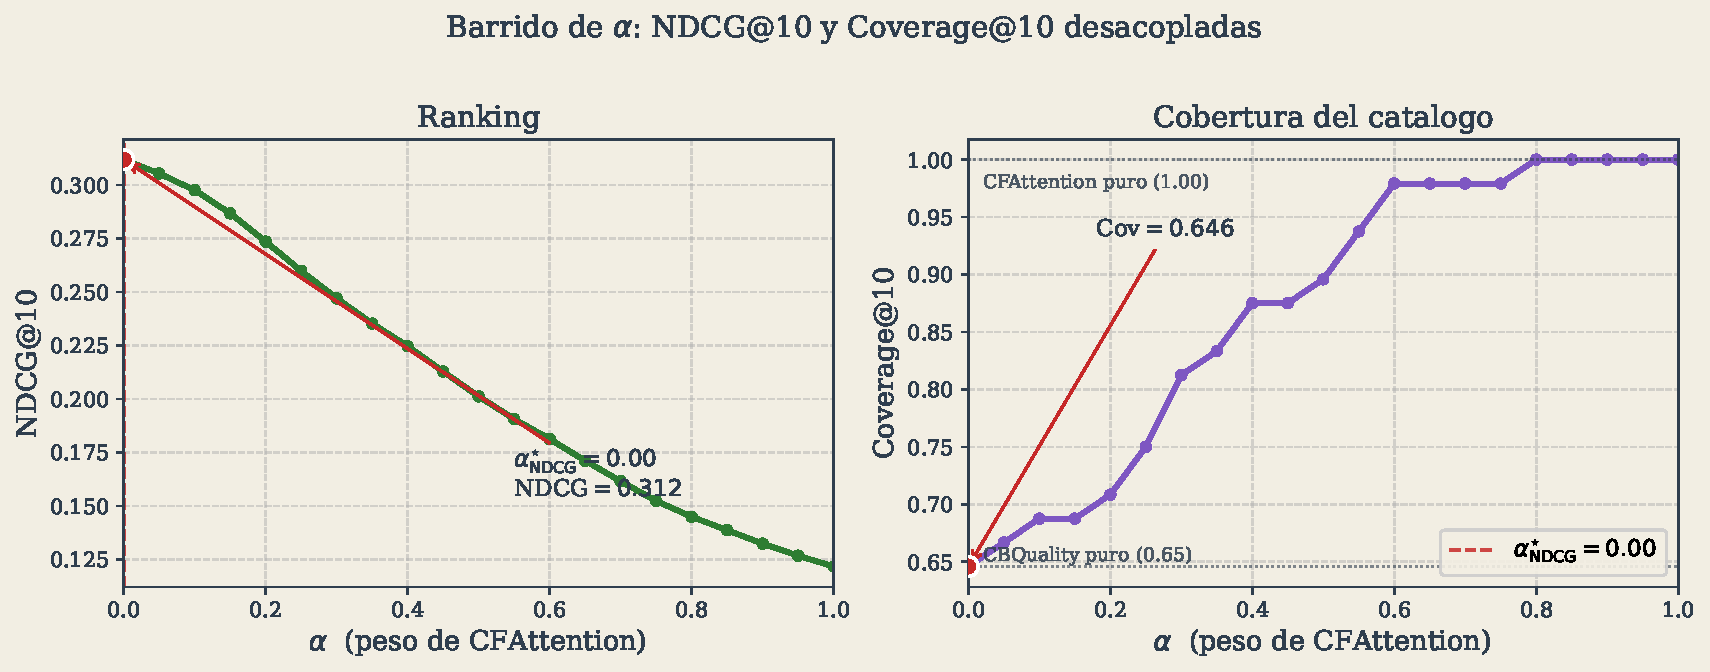
\includegraphics[width=0.52\textwidth]{alpha_metrics.pdf}
	% 	\vskip0.3ex
	% 	\raggedright
	% 	\begin{compactitem}\setlength\itemsep{0pt}
	% 		\item \textbf{NDCG@10} decrece con $\alpha$: el relevancia proviene de \texttt{CBQuality}.
	% 		\item \textbf{Cov@10} crece y satura en $1.0$: la diversidad proviene de \texttt{CFAttention}.
	% 		\item No existe un $\alpha^{*}$ \'unico: la elecci\'on depende de $\beta$
	% 		(prioridad relevancia \emph{vs.}\ cobertura).
	% 	\end{compactitem}
	% }

	%----------------------------------------------------------------------------------------
	%	8. ANALISIS DE SENSIBILIDAD
	%----------------------------------------------------------------------------------------
	\headerbox{8.\ An\'alisis de sensibilidad}{name=sensibilidad,column=1,below=modelo,span=1}{
		\centering
		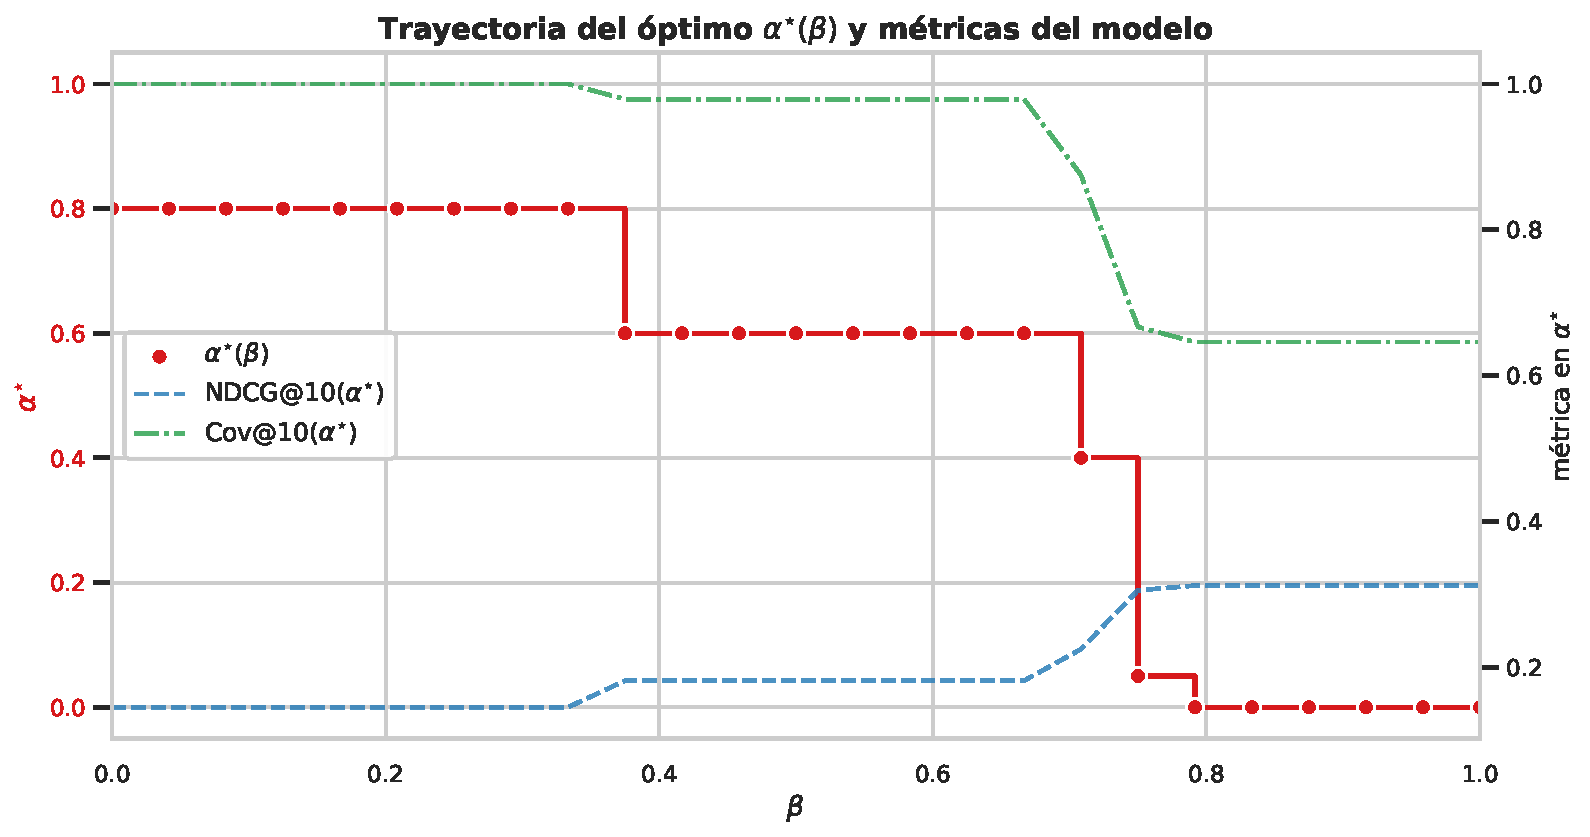
\includegraphics[width=\linewidth]{alphaVSbeta.pdf}
		\vskip0.3ex
		\raggedright\footnotesize
		Trayectoria del \'optimo $\alpha^{\star}(\beta)$ (escalera roja) y m\'etricas
		realizadas en \'el. Al priorizar \textbf{relevancia} ($\beta\!\uparrow$) el
		\'optimo \hl{migra} de un filtrado colaborativo ($\alpha^{\star}\!\approx\!0.8$) a
		un filtrado basado en contenido ($\alpha^{\star}\!\to\!0$). El eje gemelo recorre la frontera
		de Pareto: $\mathrm{Cov@10}$ cae mientras $\mathrm{NDCG@10}$ sube.
	}

	%----------------------------------------------------------------------------------------
	%	9. CONCLUSIONES
	%----------------------------------------------------------------------------------------
	\headerbox{9.\ Conclusiones}{name=conclusiones,column=1,below=sensibilidad,span=1}{
		\vspace{0.12cm}
		\begin{compactitem}\setlength\itemsep{0pt}
			\item ABSA convierte el texto libre de las rese\~nas en perfiles interpretables, tanto para los usuarios como para los pueblos.
			\item El h\'ibrido permite obtener modelos diversos que se ajustan a las necesidades del cliente; cobertura del catálogo y/o relevancia.
		\end{compactitem}
		\vspace{0.12cm}
	}

\end{poster}
\end{document}
